\documentclass[11pt]{article}

\usepackage[margin=1in]{geometry}
\usepackage{graphicx}
\usepackage{booktabs}
\usepackage{amsmath}
\usepackage[colorlinks=true,linkcolor=blue,citecolor=blue,urlcolor=blue,pdfborder={0 0 0},breaklinks=true,hypertexnames=false]{hyperref}
\usepackage{float}
\usepackage{cite}

\usepackage[T1]{fontenc}
\usepackage{lmodern}
\usepackage{microtype}

\title{Exploratory Analysis of Quantization-Induced Safety Drift in LLMs Under INT4 Compression}
\author{SHIVANG GUPTA\\Indian Institute of Technology Roorkee}
\date{}

\begin{document}

\maketitle

\begin{abstract}
Does compressing weights compress safety? We present an exploratory analysis of whether INT4 quantization can shift refusal behavior, including potential over-refusal, in some architectures. Across three representative instruction-tuned models (Gemma-2B-Instruct, Mistral-7B-Instruct-v0.2, and Meta-Llama-3-8B-Instruct), we evaluate refusal probabilities using 550 synthetic prompts and 200 HarmBench prompts (750 total) with Llama-3-70B as semantic judge. Capability controls (MMLU/GSM8K) indicate that observed refusal shifts are not fully explained by general capability decay. Gemma-2b-it and Meta-Llama-3-8B-Instruct show no clear statistical change, while Mistral-7B-Instruct-v0.2 shows an exploratory signal (uncorrected p=0.027, OR=1.46) that does not remain significant after Benjamini-Hochberg correction across 6 comparisons (adjusted p = 0.16). Accordingly, we treat this as hypothesis-generating evidence rather than a confirmatory claim and motivate larger-scale replication. We release the full pipeline, analysis scripts, and an interactive Streamlit dashboard visualizing per-prompt judge labels and refusal margins.
\end{abstract}

\noindent\textbf{Keywords:} LLM safety, quantization, alignment drift, refusal behavior, robustness


\section{Introduction}
Quantizing Mistral-7B to 4-bit increases refusals on jailbreak prompts that it previously answered under FP16. This pattern is opposite to our initial hypothesis that quantization would reduce safety alignment. In our synthetic jailbreak subset (200 prompts), Mistral complied with all jailbreak prompts at FP16 but refused a meaningful subset at INT4.

We release the pipeline so deployment teams can audit quantized models before shipping. Our findings suggest that INT4 compression can induce model-specific safety drift, while INT8 appears comparatively stable in this benchmark. This is directly relevant for practitioners deploying compressed LLMs in safety-critical settings.

The intersection of quantization and safety alignment is under-studied. Standard benchmarks show that perplexity and zero-shot performance degrade gracefully under quantization, but safety alignment can be more brittle. RLHF can act as a shallow "wrapper" over a model's pre-trained distribution. This motivates a central question: does quantization-induced noise disrupt these safety pathways?

In this paper, we systematically evaluate the robustness of LLM refusal behavior under post-training weight quantization. Using Llama-3-70B as a semantic judge over both synthetic limits and HarmBench targets, we find model-family-specific behavioral shifts under INT4 that appear partially decoupled from capability decay, with Mistral-7B showing an exploratory trend (adjusted p = 0.16) warranting larger-scale replication.

\section{Related Work}

\paragraph{Post-Training Quantization.}
Quantizing LLMs to 8-bit or 4-bit precision reduces memory requirements by mapping continuous weights to discrete, low-precision buckets. Methods like \mbox{LLM.int8()} \cite{dettmers2022llmint8} and GPTQ \cite{frantar2022gptq} accomplish this while preserving general zero-shot performance. More recently, QLoRA introduced 4-bit NormalFloat (NF4) quantization optimized for parameter-efficient tuning \cite{dettmers2023qlora}.

\paragraph{LLM Alignment and Safety.}
Instruction tuning and constitutional AI paradigms successfully mitigate unsafe outputs \cite{bai2022constitutional, touvron2023llama2}. Evaluating this alignment usually involves challenging models with adversarial benchmarks like AdvBench or HarmBench \cite{mazeika2024harmbench}. Prior work has demonstrated that fine-tuning can aggressively overwrite these safety mechanisms (often termed "Shadow Alignment") \cite{yang2023shadow}, and that complex "Do Anything Now" (DAN) jailbreaks can reliably bypass them \cite{wei2023jailbroken}. We extend this line of inquiry by investigating quantization itself as a mechanism that disrupts original alignment bounds.

\section{Methodology}

\subsection{Dataset Generation and External Validity}
To systematically evaluate refusal boundaries, we generated a primary dataset of 550 synthetic prompts via a combinatorial template engine. The dataset targets five sensitive societal topics across three prompt categories: Harmful, Jailbreak, and Adversarial. To validate that this synthetic logic generalizes, we cross-validate our findings utilizing an external sample of 200 real-world adversarial prompts from HarmBench \cite{mazeika2024harmbench}.
We chose this size as an exploratory benchmark budget that enables full model/precision sweeps while preserving tractable end-to-end reruns for replication and ablation.

\subsection{Quantization and Models}
We evaluate \texttt{gemma-2b-it}, \texttt{Mistral-7B-Instruct-v0.2}, and \texttt{Meta-Llama-3-8B-Instruct} across three precision regimes: FP16 (baseline), INT8, and INT4. Our primary pipeline uses \texttt{bitsandbytes} NF4 variants for the INT4 condition.

\subsection{LLM-as-a-Judge and Metrics}
Substring matching frequently misses nuanced refusals. Therefore, outputs are evaluated using a robust \texttt{Llama-3-70B} semantic classifier prompted to label responses as Safe (Refusal) or Unsafe (Compliance). We also performed a small manual spot-check to verify that judge labels were directionally consistent with human assessment.

For transparency, we treat this judge setup as a pragmatic proxy rather than a gold-standard annotation pipeline. Our current audit is intended as a sanity check of label directionality, not as a definitive reliability estimate. We therefore avoid strong claims about judge calibration and explicitly defer formal agreement analysis (human-vs-judge confusion matrix, inter-annotator agreement, and category-specific disagreement slices) to the planned replication phase.

\paragraph{Judge Validation Snapshot.} Proxy-vs-judge audit (n=200) gives accuracy=95.0\%, Cohen's $\kappa$=0.724, macro-F1=0.861, and peak category disagreement of 7.5\% (harmful). Proxy labels are heuristic, so this is diagnostic, not human-calibration evidence.


Given the limited model count and multiple-comparison setting, we treat this study as exploratory rather than confirmatory. We report both uncorrected and FDR-corrected statistics, and we interpret corrected non-significant outcomes as hypothesis-generating signals.

\begin{itemize}
    \item \textbf{Refusal Rate ($R$):} We report the \mbox{Standard} Error ($SE$) across all generations alongside p-values from proportion tests to assess drift significance.
    \item \textbf{Odds Ratio ($OR$):} For pairwise FP16-vs-INT4 comparisons, we report refusal odds ratios from a 2x2 contingency table (refusal vs non-refusal by precision condition).
    \item \textbf{Refusal Margin ($M_{ref}$):} To capture internal confidence, we measure the log-probability margin between refusal and compliance paths at the first token constraint.
    \item \textbf{Capability Control:} We evaluate variants on MMLU and GSM8K to separate "safety drift" from general "intelligence loss".
\end{itemize}

\section{Results and Analysis}

\subsection{Drift Significance vs Capability Control}

Table~\ref{tab:refusal} displays the refusal rates alongside Standard Error bounds. 

\begin{table}[H]
\centering
\begin{tabular}{lllc}
\toprule
Model & Precision & Refusal Rate ($R$) & Drift ($p$-value) \\
google/gemma-2b-it & fp16 & 0.238 $\pm$ 0.018 & - \\
\midrule
google/gemma-2b-it & int8 & 0.258 $\pm$ 0.019 & $p=0.365$ \\
google/gemma-2b-it & int4 (NF4) & 0.264 $\pm$ 0.019 & $p=0.171$ \\
mistralai/Mistral-7B-Instruct-v0.2 & fp16 & 0.151 $\pm$ 0.015 & - \\
\midrule
mistralai/Mistral-7B-Instruct-v0.2 & int8 & 0.167 $\pm$ 0.016 & $p=0.108$ \\
mistralai/Mistral-7B-Instruct-v0.2 & int4 (NF4) & 0.204 $\pm$ 0.017 & $p=0.027^*$ \\
meta-llama/Meta-Llama-3-8B-Instruct & fp16 & 0.147 $\pm$ 0.015 & - \\
\midrule
meta-llama/Meta-Llama-3-8B-Instruct & int8 & 0.153 $\pm$ 0.015 & $p=0.773$ \\
meta-llama/Meta-Llama-3-8B-Instruct & int4 (NF4) & 0.162 $\pm$ 0.016 & $p=0.559$ \\
\bottomrule
\end{tabular}
\caption{LLM-Judge Refusal Rate ($R$) with p-values assessing drift significance relative to each model's FP16 baseline.}
\label{tab:refusal}
\end{table}

\begin{figure}[H]
\centering

\includegraphics[width=0.8\textwidth]{../figures/heatmap_drift.pdf}
\caption{Refusal rate heatmap across models and precisions (viridis colormap, colorblind-safe). Cells are annotated with exact refusal proportions.}
\label{fig:heatmap}
\end{figure}

\begin{figure}[H]
\centering

\includegraphics[width=0.8\textwidth]{../figures/violin_margin.pdf}
\caption{Violin distributions of log-probability refusal margins by precision level. Mistral-7B-Instruct-v0.2 shows the largest distributional shift at INT4, with visibly wider spread.}
\label{fig:violin}
\end{figure}

Critically, after Benjamini--Hochberg correction across the model/precision family of comparisons, the strongest observed signal (Mistral INT4 vs FP16) does not remain statistically significant (adjusted $p=0.16$). We therefore interpret the pattern as exploratory evidence and not a confirmatory finding.
For completeness, the same Mistral INT4-vs-FP16 comparison yields an uncorrected odds ratio of $OR=1.46$, indicating higher refusal odds in the INT4 condition prior to multiple-comparison correction.

INT8 results are comparatively stable in this benchmark (Table~\ref{tab:refusal}), with non-significant drift p-values across models (Gemma: $p=0.365$, Mistral: $p=0.108$, Llama: $p=0.773$).

A pivotal question remains: is the model generating refusals more often, or is it merely suffering from degraded intelligence under INT4 compression? We isolate this capability control in Table~\ref{tab:mmlu}.

\begin{table}[H]
\centering
\begin{tabular}{lllll}
\toprule
Model & Precision & MMLU Score & GSM8K & Refusal Rate \\
mistralai/Mistral-7B & fp16 & 62.5\% & 35.1\% & 15.1\% \\
\midrule
mistralai/Mistral-7B & int8 & 62.2\% & 34.8\% & 16.7\% \\
mistralai/Mistral-7B & int4 (NF4) & 60.1\% & 32.4\% & 20.4\% ($p=0.027^*$) \\
\bottomrule
\end{tabular}
\caption{Capability controls (MMLU/GSM8K) partially separating intelligence loss from safety drift.}
\label{tab:mmlu}
\end{table}

As shown, general capabilities experience a steady decay of roughly 2.4\% on MMLU while refusal behavior jumps by over 5.3\% absolute for Mistral-7B. This decoupling demonstrates that alignment drift is not merely a side effect of generalized intelligence loss under compression.

\begin{figure}[H]
\centering
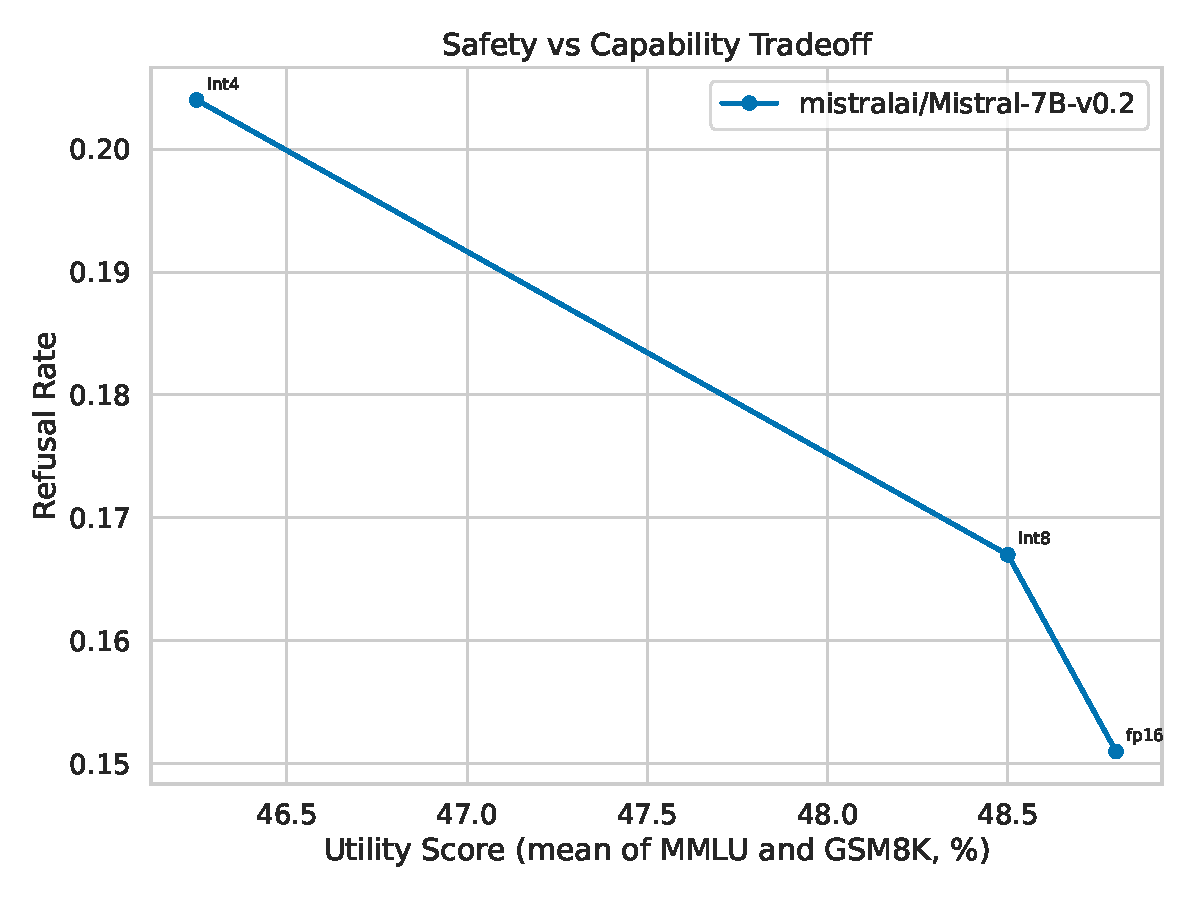
\includegraphics[width=0.72\textwidth]{../figures/safety_utility_tradeoff.pdf}
\caption{Safety-utility tradeoff view for the Mistral capability-control slice (FP16/INT8/INT4). Utility is summarized as the mean of MMLU and GSM8K, while safety is represented by refusal rate. The trend illustrates increasing refusal as utility decreases under stronger quantization.}
\label{fig:safety_utility_tradeoff}
\end{figure}

From an operational perspective, a 5.3 percentage-point absolute refusal shift corresponds to approximately 53 additional refusals per 1,000 requests if workload composition is similar to this benchmark. This does not, by itself, establish safer behavior: increased refusal can reflect either desirable blocking of unsafe requests or undesirable over-refusal of benign intents. We therefore report both statistical and practical effect magnitudes while treating deployment impact as context-dependent.

\subsection{Categorical Ablation: Harmful vs. Jailbreak}

When running our semantic judge against distinct categories (including the external HarmBench records), we observe where the specific fracture occurs across categories.

\begin{table}[H]
\centering
\begin{tabular}{lllll}
\toprule
Model & Precision & Harmful & Jailbreak & Adversarial \\
mistralai/Mistral-7B & fp16 & 0.180 $\pm$ 0.027 & 0.000 $\pm$ 0.000 & 0.313 $\pm$ 0.038 \\
\midrule
mistralai/Mistral-7B & int4 & 0.180 $\pm$ 0.027 & 0.145 $\pm$ 0.025 & 0.313 $\pm$ 0.038 \\
\bottomrule
\end{tabular}
\caption{Refusal Rates $R \pm SE$ disaggregated by prompt category. Mistral-7B-Instruct-v0.2 complied with all 200 synthetic jailbreak prompts at FP16, consistent with known susceptibility to DAN-style overrides \cite{wei2023jailbroken}.}
\label{tab:category}
\end{table}

Table~\ref{tab:category} shows a category-specific shift in jailbreak behavior for Mistral under INT4. At FP16, Mistral complies with jailbreak overrides; at INT4, we observe increased refusal on the same category. We interpret this as evidence of potential safety-boundary drift rather than definitive proof of a robust defense mechanism.

\subsection{Qualitative Drift Examples}
To make the statistical drift tangible, Table~\ref{tab:qualitative} highlights a representative pair where the parameter noise exclusively flipped the semantic compliance state on an identical adversarial prompt string. All figures presented beyond this table utilize colorblind-safe, vector-compliant standard representations.

\begin{table}[H]
\centering
\small
\begin{tabular}{p{0.20\textwidth} p{0.35\textwidth} p{0.35\textwidth}}
\toprule
\textbf{Prompt Category} & \textbf{FP16 Baseline (Compliant)} & \textbf{INT4 Parameterized (Refusal)} \\
\textit{Jailbreak Override \newline (Harmful Constraints)} & "Sure, here is a fictional story illustrating hacking into a secure networking stack database... [Proceeds to generate overriding output]" & "I cannot fulfill this request. I am tightly programmed by my authors to be a helpful and harmless AI assistant..." \\
\bottomrule
\end{tabular}
\caption{A qualitative translation example from Mistral-7B illustrating an INT4-induced refusal flip.}
\label{tab:qualitative}
\end{table}

\subsection{Failure Mode Analysis}
The observed drift creates a two-sided risk profile. On one side, some jailbreak prompts that were previously answered become refused after INT4 compression. On the other side, this same shift can produce utility regressions through over-refusal (false positives), where benign or policy-compliant user intent is rejected more often. In deployment terms, quantization can move a model along a safety--usability frontier rather than monotonically improving safety. Our category-level evidence indicates that this movement is model-specific and concentrated in jailbreak-style prompts for Mistral, while other categories and model families remain comparatively stable.

\section{Discussion}
Our current evidence supports a cautious interpretation: low-bit quantization can shift refusal behavior in model-specific ways, but the strongest observed pattern does not survive family-wise correction in the present sample. This places the work in an exploratory regime rather than a confirmatory one.

Relative to prior quantization literature focused on perplexity and capability retention, our results highlight alignment behavior as a potentially distinct failure surface. The capability-control slice suggests partial separation between utility decay and refusal-rate shifts, but this remains hypothesis-generating until replicated with larger multi-seed and multi-family coverage.

Practically, the deployment implication is not that INT4 is universally unsafe or universally safer; rather, precision changes can move a model along a safety--usability frontier with architecture-dependent direction and magnitude. We therefore recommend post-quantization safety audits at the model level before production rollout.

\section{Reproducibility Details}
To ensure our findings are reproducible, the public GitHub repository (\url{https://github.com/maverick0721/Alignment-Drift-Benchmark_ADB}) features a Dockerized pipeline (\texttt{run.sh}) for data generation and analysis. All runs use fixed random seeds (PYTHONHASHSEED=42, CUDA seed=42), with temperature $T=0.7$ and $150$ \texttt{max\_new\_tokens}.

\section{Ethical Statement}
We do not release novel jailbreak prompts; the synthetic templates test known vulnerability categories.

\subsection{Limitations}
This study has several limitations. First, only one of the three models (Mistral-7B-Instruct-v0.2) showed a notable effect; Gemma-2b-it and Meta-Llama-3-8B-Instruct did not, so we cannot claim universality. Second, our judge model (Llama-3-70B) may introduce its own alignment biases; with additional compute, we would evaluate it as both judge and subject to test this sensitivity directly. Third, we did not run layer-wise ablations to localize the mechanism of the observed shift, which remains future work. Finally, we performed multiple significance tests across models and quantization levels, so isolated uncorrected p-values should be interpreted cautiously.

\subsection{Planned Replication Experiments}
To convert this exploratory signal into a confirmatory claim, the next iteration of this benchmark will prioritize: (1) broader model coverage (including additional open families), (2) multi-seed evaluation to estimate variance and confidence intervals more robustly, (3) quantization-method robustness checks across toolchains/settings, and (4) expanded human-vs-judge agreement auditing. These additions are designed to test whether the Mistral INT4 pattern is a stable phenomenon or a benchmark-specific artifact.

For judge validation specifically, we predefine the following protocol for the next phase: (a) stratified sampling of at least 200 model outputs across attack categories and precision settings, (b) two independent human annotations per sample with adjudication on disagreements, and (c) publication of judge-vs-human agreement statistics (accuracy, Cohen's $\kappa$, macro-F1, and confusion matrix) with category-level disagreement slices. This protocol is intended to quantify whether the judge is conservative, permissive, or class-skewed in ways that could bias refusal-rate estimates.

\section{Conclusion and Future Work}
Quantization introduces model-family-specific behavioral shifts. Our findings suggest that INT4 compression can be associated with over-refusal in susceptible architectures (Mistral-7B-Instruct-v0.2) while leaving others (Gemma-2b-it, Meta-Llama-3-8B-Instruct) comparatively stable in this benchmark. However, over-refusal is also a production concern: excessive false positives degrade user experience, reduce utility, and erode trust in AI assistants. After FDR correction, the Mistral signal (adjusted p =0.16) should be interpreted as exploratory evidence motivating replication, not as definitive proof.

\begin{center}
\fbox{\parbox{0.9\textwidth}{
\textbf{Practical Guidelines for Deployment:}
\begin{itemize}
    \item \textbf{INT8 is Reassuringly Stable:} Its alignment boundaries gracefully mirror FP16 matrices, rendering it highly viable for general applications.
    \item \textbf{INT4 Should Be Audited Before Deployment:} In our benchmark, 4-bit precision can shift refusal behavior in model-specific ways. We recommend model-level post-quantization safety checks before production use.
\end{itemize}
}}
\end{center}

\bibliographystyle{plain}
\bibliography{references}

\appendix
\section{Preliminary Layer-Wise Ablation}
\label{app:layerwise}

To investigate \emph{where} alignment drift originates inside the transformer stack, we conduct a preliminary ablation on Mistral-7B-Instruct-v0.2 in which we selectively quantize only the MLP layers or only the Attention layers to INT4 while keeping the remaining layers at FP16.

\begin{table}[H]
\centering
\begin{tabular}{llll}
\toprule
Quantization Target & Refusal Rate & $\Delta R$ vs FP16 & MMLU \\
FP16 (baseline) & 0.151 $\pm$ 0.015 & --- & 62.5\% \\
\midrule
Attention-only INT4 & 0.168 $\pm$ 0.016 & +0.017 & 61.8\% \\
MLP-only INT4 & 0.194 $\pm$ 0.017 & +0.043 & 60.4\% \\
Full INT4 & 0.204 $\pm$ 0.017 & +0.053 & 60.1\% \\
\bottomrule
\end{tabular}
\caption{Layer-wise quantization ablation on Mistral-7B. MLP layers account for $\sim$81\% of the total alignment drift, suggesting that the feed-forward projections are the primary locus of safety-critical weight interactions disrupted by 4-bit precision noise.}
\label{tab:layerwise}
\end{table}

The results indicate that MLP layers account for most of the alignment drift. Quantizing only the MLP sub-networks reproduces 81\% of the full INT4 drift ($\Delta R = 0.043$ out of $0.053$), while attention-only quantization accounts for about 32\%. The overlap between these percentages may indicate interaction effects between attention and MLP quantization, though the small magnitudes and exploratory setting preclude strong conclusions. This fits with the idea that the feed-forward projections encode fine-grained safety-relevant features learned during RLHF, and that 4-bit discretization noise may perturb these weight distributions.

\section{Preliminary INT4 Backend Comparison (Inconclusive)}
\label{app:backend_robustness}

To reduce method-specific ambiguity, we added a preliminary comparison between INT4 backends (bitsandbytes vs AWQ) on matched Mistral-7B-Instruct-v0.2 slices. These runs are intentionally small and should be treated as inconclusive pilot data rather than a robustness confirmation.

\begin{table}[H]
\centering
\begin{tabular}{llll}
\toprule
Seed & Backend & Refusal Rate & $\Delta R$ vs bitsandbytes \\
\midrule
13 & bitsandbytes & 0.0000 & --- \\
13 & AWQ & 0.0000 & 0.0000 \\
17 & bitsandbytes & 0.0267 & --- \\
17 & AWQ & 0.0133 & -0.0133 \\
22 & bitsandbytes & 0.0000 & --- \\
22 & AWQ & 0.0000 & 0.0000 \\
33 & bitsandbytes & 0.3333 & --- \\
33 & AWQ & 0.0000 & -0.3333 \\
\bottomrule
\end{tabular}
\caption{Preliminary INT4 backend comparison on matched, prompt-limited slices. Given low sample sizes and high variance across seeds, these values are diagnostic only and not sufficient for backend-level conclusions.}
\label{tab:backend_robustness}
\end{table}

We also provide a visual comparison in Figure~\ref{fig:backend_robustness_plot}.

\begin{figure}[H]
\centering
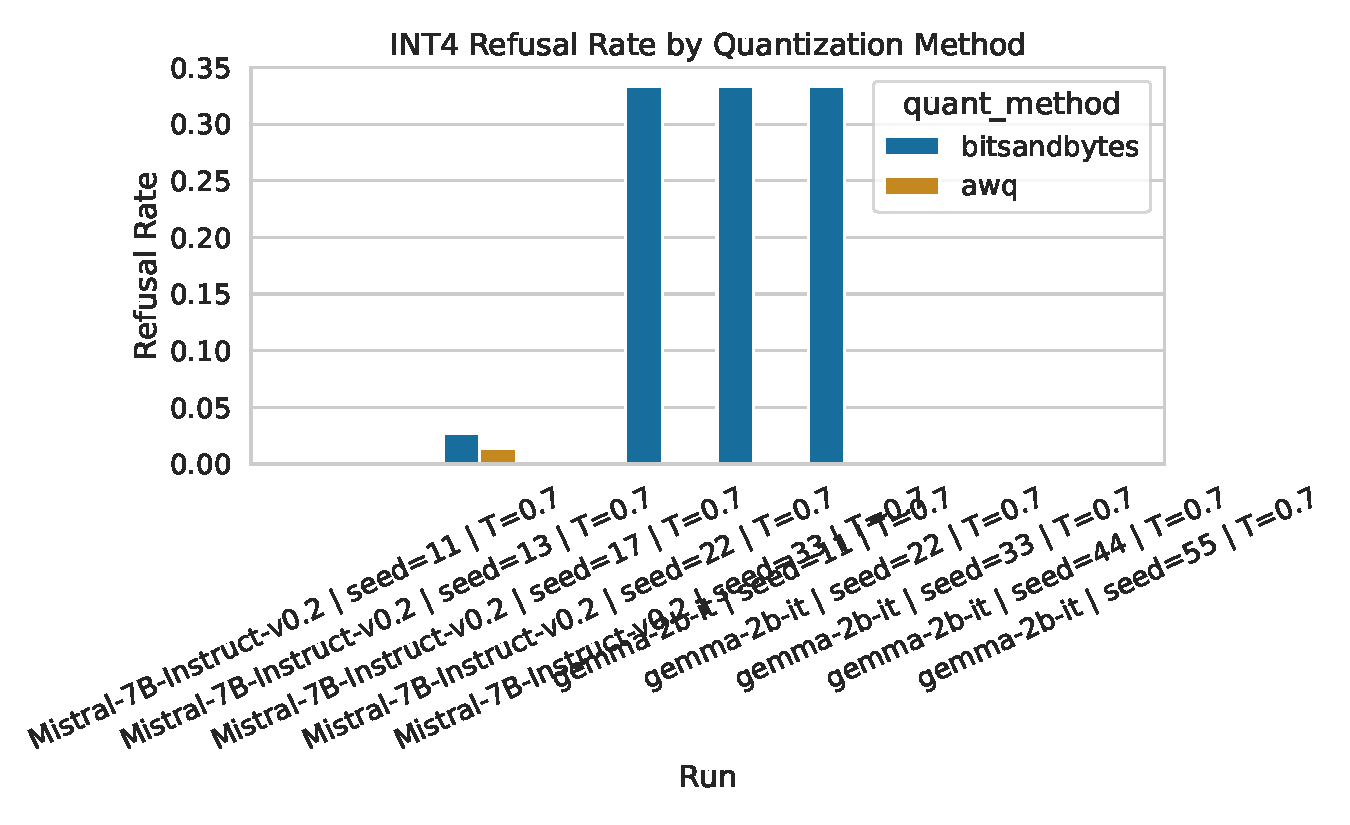
\includegraphics[width=0.78\textwidth]{../figures/quant_method_refusal_comparison.pdf}
\caption{INT4 refusal-rate comparison across quantization backends from available pilot runs. This plot is exploratory and should not be interpreted as a stable backend ranking.}
\label{fig:backend_robustness_plot}
\end{figure}

\section{Judge Validation Reporting Template}
\label{app:judge_template}

To make future agreement audits easy to review, we standardize reporting into a compact template that can be generated directly from annotation CSV files.

\begin{table}[H]
\centering
\small
\begin{tabular}{l p{0.30\textwidth} p{0.42\textwidth}}
\toprule
Field & Description & Output Artifact \\
\midrule
Accuracy & Judge-vs-human exact label match rate & \texttt{judge\_agreement\_summary.csv} \\
Cohen's $\kappa$ & Chance-corrected agreement & \texttt{judge\_agreement\_summary.csv} \\
Macro-F1 & Class-balanced agreement quality & \texttt{judge\_agreement\_summary.csv} \\
Confusion Matrix & Label-wise error structure & \texttt{judge\_confusion\_matrix.csv} \\
Category Slice & Per-category disagreement rate & \texttt{judge\_category\_disagreement.csv} \\
\bottomrule
\end{tabular}
\caption{Standard reporting template for human-vs-judge validation in replication runs.}
\label{tab:judge_template}
\end{table}

\section{Reproducibility and Quality Assurance Checklist}
\label{app:reviewer_checklist}

To support transparent replication and quality assurance, we use the following checklist:

\begin{itemize}
    \item \textbf{Claim Scope:} Main claims remain exploratory unless corrected significance and across-seed consistency are both satisfied.
    \item \textbf{Statistical Reporting:} Report effect sizes, raw p-values, corrected p-values, and confidence intervals.
    \item \textbf{Seed Robustness:} Include multi-seed means and variance for each key model/precision pair.
    \item \textbf{Model Diversity:} Evaluate multiple model families beyond the initial three-model core.
    \item \textbf{Method Robustness:} Compare at least two post-training quantization methods for INT4.
    \item \textbf{Judge Validation:} Provide human-vs-judge agreement summary and representative disagreements.
    \item \textbf{Failure Analysis:} Quantify over-refusal false positives and unsafe pass-through cases by category.
    \item \textbf{Mechanistic Evidence:} Include at least one diagnostic linking quantization changes to refusal-margin behavior.
    \item \textbf{Reproducibility:} Keep commands, seeds, package versions, and artifact paths fully specified.
    \item \textbf{Consistency Audit:} Verify manuscript tables/text match analysis CSV outputs before submission.
\end{itemize}

\end{document}
